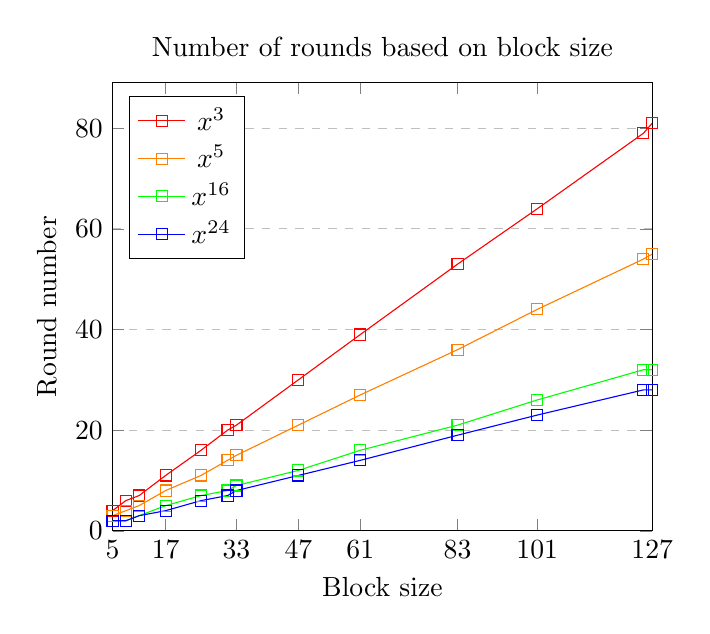
\begin{tikzpicture}
    \centering
    \begin{axis}[
        title={Number of rounds based on block size},
        xlabel={Block size},
        ylabel={Round number},
        xmin=5, xmax=127,
        ymin=0,
        xtick={5,17,33,47,61,83,101,127},
        legend pos=north west,
        ymajorgrids=true,
        grid style=dashed,
    ]
    
    \addplot[color=red,mark=square]
        coordinates {((5,4)(8,6)(11,7)(17,11)(25,16)(31,20)(33,21)(47,30)(61,39)(83,53)(101,64)(125,79)(127,81)};
        \addlegendentry{$x^3$}
        
    \addplot[color=orange,mark=square]
        coordinates {(5,3)(8,4)(11,5)(17,8)(25,11)(31,14)(33,15)(47,21)(61,27)(83,36)(101,44)(125,54)(127,55)};
        \addlegendentry{$x^5$}
        
    \addplot[color=green,mark=square]
        coordinates {(5,2)(8,2)(11,3)(17,5)(25,7)(31,8)(33,9)(47,12)(61,16)(83,21)(101,26)(125,32)(127,32)};
        \addlegendentry{$x^{16}$}

    \addplot[color=blue,mark=square]
        coordinates {(5,2)(8,2)(11,3)(17,4)(25,6)(31,7)(33,8)(47,11)(61,14)(83,19)(101,23)(125,28)(127,28)};
        \addlegendentry{$x^{24}$}
        
    \end{axis}
\end{tikzpicture}